\section{Sistemas de partículas}

    \capequation{Cantidad de movimiento lineal}
        \begin{equation}
            \vec{P} = m \cdot \vec{v}        
        \end{equation}
        \begin{itemize}
        \item Otros nombres posibles...
            \begin{itemize}
            \item Momento lineal
            \item Momento traslacional
            \item Cantidad de movimiento lineal
            \item Cantidad de movimiento
            \item Impetu
            \item Momentum
            \item Momento
            \end{itemize}
        \end{itemize}
        
    \capequation{Variación de la cantidad de movimiento lineal}
        \begin{equation}
            \frac{d\vec{P}}{dt} = \vec{F}
        \end{equation}

    \capequation{Fuerza media}
        \begin{equation}
            F_{med} = \frac{\Delta P}{\Delta T}
        \end{equation}
    
    \capequation{Conservación de $\vec{P}$}
        \begin{equation}
            \sum \vec{F}_{ext}=\vec{0} \rightarrow \vec{P}=cte \rightarrow \vec{v}=cte \rightarrow \vec{a}=\vec{0}
        \end{equation}
    
    \capequation{Impulso lineal}
        \begin{equation}
            \vec{I}=\int_{t_1}^{t_2} \Vec{F} \boldsymbol{\cdot} d\vec{t}
        \end{equation}
        \begin{equation}
            \vec{I} = \Delta \vec{P}        
        \end{equation}
    
    \capequation{Torque de una fuerza}
        \begin{equation}
            \overrightarrow{\tau_{\vec{F}}^{o}} = \vec{r}_o \times \vec{F}
        \end{equation}
        \begin{equation}
            \left|{\tau_{\vec{F}}^{o}}\right| = F \cdot r_o \cdot \sin{(\alpha)} = F \cdot d
        \end{equation}
        
        \begin{center}
        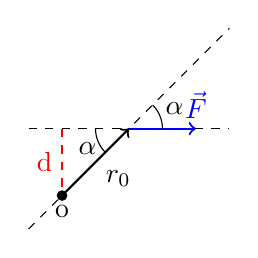
\begin{tikzpicture}[scale=0.85]
            \draw[dashed] (-1.5,0) -- (1.5,0);
            \draw[dashed] (-1.5,-1.5) -- (1.5,1.5);
            \draw[dashed,red] (-1,0) -- (-1,-1) node[anchor=east] at (-1,-0.5){d};
            \draw[thick,blue,->] (0,0) -- (1,0) node[anchor=south]{$\vec{F}$} ;
            \draw[thick,->] (-1,-1) -- (0,0) node[anchor=west] at (-0.5,-0.75){$r_0$};
            \filldraw[black] (-1,-1) circle (2pt) node[anchor=north]{o};
            \draw (0.5,0) arc (0:45:0.5) node[anchor=west] at (0.4,0.3){$\alpha$};
            \draw (-0.5,0) arc (0:45:-0.5)  node[anchor=west] at (-0.9,-0.3){$\alpha$};
        \end{tikzpicture}
        \end{center}
        \begin{itemize}
            \item \textit{d}: Brazo de palanca
            \item Otros nombres posibles (tener especial cuidado en el contexto en el que se emplean dada la similitud con los nombres alternativos de $\vec{P}$) ...
                \begin{itemize}
                    \item Fuerza rotacional
                    \item Efecto de rotación
                    \item Torca
                    \item \textit{Momento de fuerza} 
                    \item \textit{Momento}
                    \item \textit{Par motor} (específica del área mecánica)
                \end{itemize}
            \item \textbf{Fuerza Central}: Son aquellas que realizan un torque nulo respecto de un punto de referencia. (Ej: fuerzas que ``pasan'' por el punto de referencia de torques)
            \item \textbf{Cuplas}: Par de fuerzas separadas a una distancia d, de igual intensidad, misma dirección y sentidos opuestos, donde cuyo valor en módulo es $F\cdot d$. Es una herramienta útil para desacoplar el movimiento de roto-traslación de un sistema como la suma de un movimiento de traslación y uno de rotación
        \end{itemize}
        \begin{center}
            \begin{tikzpicture}
                %Axis
                \draw[->] (0,-1.25)--(0,1.25) node[above] {y};
                \draw[->] (0,0)--(3,0) node[above] {x};
                %r1 r2
                \draw[britishracinggreen,thick,->] (0,0)--(1,0) node[above] at (0.5,0) {$r_1$};
                \draw[britishracinggreen,thick,->] (1,0)--(2,0) node[above] at (1.5,0) {$r_2$};
                %Forces
                \draw[blue,thick,->] (1,0)--(1,1) node[above] {$F_1$};
                \draw[blue,thick,->] (2,0)--(2,-1) node[below] {$F_2$};
                %Distance
                \draw[red,dashed] (1,-0.5)--(2,-0.5) node[above] at (1.5,-0.5) {d};
                \draw[dashed] (1,0)--(1,-1);
            \end{tikzpicture}
        \end{center}
            
    \capequation{Cantidad de movimiento angular}
        \begin{equation}
            \vec{L}^o = \vec{r}_o \times \vec{P}_o
        \end{equation}
        \begin{equation*}
            \vec{L}^o = \vec{r}_o \times m\cdot \vec{v}
        \end{equation*}
        \begin{itemize}
            \item Otros nombres posibles (tener especial cuidado en el contexto en el que se emplean dada la similitud con los nombres alternativos de $\vec{L}$) ...
            \begin{itemize}
                \item Momento angular
                \item Momento cinético
                \item Momento rotacional
                \item Momento de momentum 
            \end{itemize}
        \end{itemize}
    
    \capequation{Variación de la cantidad de movimiento angular}
        \begin{equation}
            \frac{d\vec{L}^o}{dt} = \overrightarrow{\tau_{\vec{F}}^{o}}
        \end{equation}
    
    \capequation{Conservación de $\vec{L}^o$}
        \begin{equation}
            \sum \overrightarrow{\tau_{\vec{F}_{ext}}^{o}}=\vec{0} \rightarrow \vec{L}^o=cte \rightarrow \vec{\omega}=cte \rightarrow \vec{\gamma}=\vec{0}
        \end{equation}
        
    
            
    \capequation{Posición del centro de masa}  
        \begin{equation}
            \vec{r}_{cm} = \sum_{i=1}^{n} \frac{\vec{r}_i\cdot m_i}{M}
        \end{equation}
    
    \capequation{Velocidad del centro de masa}  
        \begin{equation}
            \vec {v}_{cm} = \sum_{i=1}^{n} \frac{\vec{v}_i\cdot m_i}{M}
        \end{equation}

    \newpage
    
    \capequation{Aceleración del centro de masa}  
        \begin{equation}
            \vec {a}_{cm} = \sum_{i=1}^{n} \frac{\vec{a}_i\cdot m_i}{M}
        \end{equation}
        
    \capequation{Cantidad de movimiento lineal del SP} 
        \begin{equation}
            \vec{P}_{sist} = \vec {P}_{cm} = {M} \cdot \vec{v}_{cm} = \sum_{i=1}^{n} \vec{v}_{i} \cdot m_i
        \end{equation}
    
    \capequation{Cantidad de movimiento angular del SP} 
        \begin{equation}
            \vec{L}_{sist}^o = \sum_{i=1}^{n} \vec{L}_{i}^o = \sum_{i=1}^n \overrightarrow{r_{i}^o} \times \overrightarrow{P_{i}^o}
        \end{equation}
        
    \capequation{Cantidad de movimiento angular (Orbital y Spin)} 
        \begin{equation}
            \begin{split}
                \vec{L}_{sist}^o &= \sum_{i=1}^{n} \vec{L}_{i}^{cm} + \overrightarrow{r}_{cm}^o \times \overrightarrow{P}_{cm}^o\\
                \vec{L}_{sist}^o &= \vec{L}_{sist}^{cm} + \vec{L}_{cm}^o\\
                \vec{L}_{sist}^o &= \vec{L}_{spin} + \vec{L}_{orbital}\\
            \end{split}
        \end{equation}
    
    \capequation{Energía potencial gravitatoria de un SP}
        \begin{equation}
            Ep = M \cdot g \cdot h_{cm}
        \end{equation}    
    
    \capequation{Energía cinética de un SP}
        \begin{equation}
            Ec_{sist}^o = \sum_{i=1}^{n} \frac{1}{2} \cdot m_i \cdot {(v_i^o)}^2
        \end{equation}
        
    \capequation{E. cinética (Orbital y Spin) - Teorema de König's} 
        \begin{equation}
        \begin{split}
            Ec_{sist}^{o} & = \frac{1}{2} \cdot M \cdot (v_{cm})^2 + \frac{1}{2} \sum_{i=1}^{n} \cdot m_i \cdot (v_i^{cm})^2\\
            Ec_{sist}^o & =  Ec_{cm}^o + Ec_{sist}^{cm}\\
            Ec_{sist}^o & = Ec_{_{orbital}} + Ec_{_{spin}}
        \end{split}
        \end{equation}
    
    \capequation{Tipos de interacciones}
        \begin{itemize}
            \item Perfectamente elástico $\rightarrow Ec^f = Ec^o \rightarrow \Delta Ec = 0$
            \item Perfectamente plástico $\rightarrow \vec{v}_{fa} = \vec{v}_{fb} $
            \item Inelástico / Endoérgico $\rightarrow Ec^f < Ec^o$
            \item Explosivo / Exoérgico $\rightarrow Ec^f > Ec^o $
        \end{itemize}
        
    \capequation{Coeficiente de restitución}
        \begin{equation}
            (\vec{v}_{2}^f-\vec{v}_{1}^f) = -e \cdot (\vec{v}_{2}^{\ o}-\vec{v}_{1}^{\ o})
        \end{equation}
        \begin{itemize}
            \item e = 1 (Perfectamente Elástico)
            \item e = 0 (Perfectamente Plástico)
            \item 0$<$e$<$1 (Inelástico / Endoérgico)
            \item e $>$ 1 (Explosivo / Exoérgico)
        \end{itemize}